\documentclass{book}
\usepackage[spanish,mexico]{babel}
\usepackage[utf8]{inputenc}
\usepackage{graphicx}
\usepackage{listings}
\usepackage{booktabs}
\usepackage{float}
\usepackage{hyperref}
\usepackage{xr}

\lstset{
    inputencoding=utf8,
    extendedchars = true,
    basicstyle=\ttfamily\small,
    keywordstyle=,
    stringstyle=,
    commentstyle=,
    breaklines=true,
    numbers=none
}

\newfloat{codigo}{H}{loc}[chapter]
\floatname{codigo}{Código}

\begin{document}

\chapter*{Paquete \texttt{Float}}\label{ch:float}
EL paquete \texttt{Float} facilita el manejo de los entornos flotantes en el documento, permitiendo controlar su ubicación con precisión, la creación de nuevos tipos de flotantes y la personalización de sus índices.

\section{Control de ubicación}\label{sec:ubicacion_float}
El parámetro \texttt{'H'}, permite forzar la colocación del flotante exactamente en el lugar donde se declara, sin que \LaTeX lo acomode automáticamente.

\subsection*{Posición preferida '\texttt{h}'}
El parámetro \texttt{h} indica que el flotante debe intentar colocarse "aquí", en el lugar donde fue declarado. Sin embargo, si no hay suficiente espacio, \LaTeX\ lo moverá automáticamente a otra posición. Si \LaTeX\ determina que no es posible colocar el flotante aquí, lo moverá al lugar más adecuado, por ejemplo, al incio de la siguiente página.

\vspace{1.5cm} % Espaciado para ilustrar cómo el flotante puede desplazarse.

\begin{figure}[h]
    \centering
    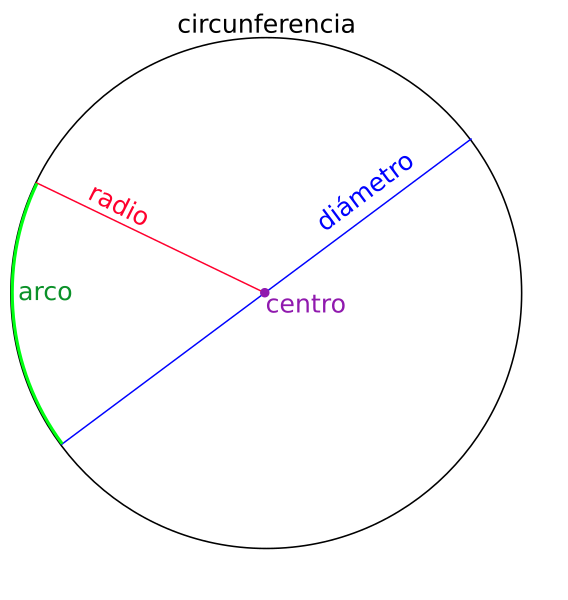
\includegraphics[scale=.2]{imagen-ejemplo.png}
    \caption{Figura usando \texttt{h}.}
    \label{fig:h}
\end{figure}



\subsection*{Posición exacta '\texttt{H}'}
El parámetro \texttt{H} fuerza a que el flotante permanezca exactamente en el lugar donde se encuentra en el código. 

\begin{figure}[H]
    \centering
    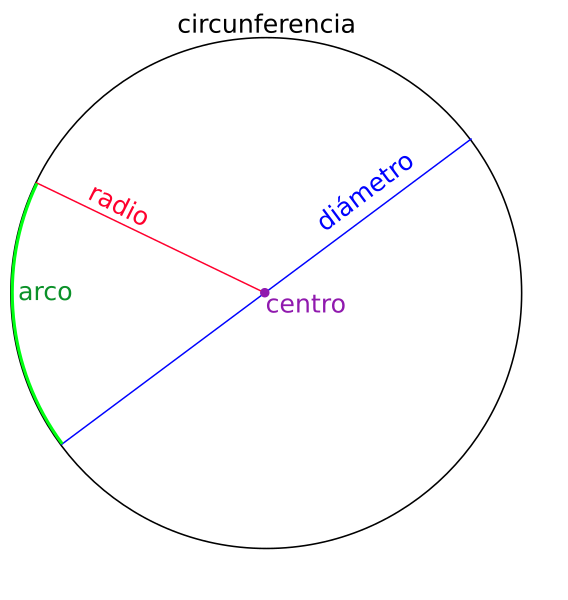
\includegraphics[scale=.2]{imagen-ejemplo.png}
    \caption{Figura usando \texttt{H}.}
    \label{fig:H}
\end{figure}

\section{Creación de nuevos flotantes}\label{sec:nuevos_flotantes}
Utilizamos \verb|\newfloat| para definir un nuevo tipo de flotante.\\

\textbf{Sintaxis:}
\begin{codigo}[H]
\centering
\begin{lstlisting}[language=LaTeX]
\newfloat{tipo}{posicion}{extension}[entorno]
\end{lstlisting}
\caption{Sintaxis para crear un nuevo estilo de float.}
\label{sintaxis:newfloat}
\end{codigo}

\begin{itemize}
    \item \texttt{nombre}: Nombre del nuevo flotante.
    \item \texttt{posicion}: Posición del flotante en la página (\texttt{t}, \texttt{b}, \texttt{h}, \texttt{p}, \texttt{H}).
    \item \texttt{extensión}: Extensión para el índice.
    \item \texttt{entorno}: Relación con otro entorno existente (capítulo, sección, subsección,...).
\end{itemize}

\subsection*{Ejemplo:}

 Creamos un nuevo tipo de flotante para algoritmos.

\begin{codigo}
    \begin{lstlisting}
        \usepackage{float}
        \newfloat{algoritmo}{htbp}{loa}[chapter]

        \begin{document}

        \begin{algoritmo}[H]
            \centering
            \caption{Algoritmo de ejemplo.}
            \label{alg:ejemplo}
        \end{algoritmo}

        \end{document}
    \end{lstlisting}
    \label{ejemplo:newfloat}
\end{codigo}


\section{Índice para nuevos flotantes}

El paquete permite generar índices específicos para los nuevos flotantes usando \verb|\listof|. 

\subsubsection*{Ejemplo:}
Generamos un índice para los elementos del nuevo tipo de flotantes.
\begin{codigo}
\begin{lstlisting}
    \usepackage{float}
        \newfloat{algoritmo}{htbp}{loa}[chapter]

        \begin{document}
        
        \listof{algoritmo}{Índice de Algoritmos}
        
        \begin{algoritmo}[H]
            \centering
            \caption{Algoritmo de ejemplo.}
            \label{alg:ejemplo}
        \end{algoritmo}

        \end{document}
\end{lstlisting}
\label{ejemplo:indice_personalizado}
\end{codigo}





\end{document}


